\documentclass{article}
\usepackage{xeCJK}
    \xeCJKsetup{AutoFakeBold=true, AutoFakeSlant=true}
    \setCJKmainfont{標楷體}
    \setmainfont{Times New Roman}
\usepackage{setspace}
    \onehalfspace
\setlength{\parskip}{1ex plus 0.5ex minus 0.2ex}
\usepackage[
top    = 2cm,
bottom = 2cm,
left   = 2.50cm,
right  = 2.50cm]{geometry}
\usepackage{mathtools}
\usepackage{physics}
\usepackage{siunitx}
    \sisetup{
        list-final-separator = { 和 }, 
        list-pair-separator = { 和 },
        range-phrase = { 至 }
    }
\usepackage{listings}
\usepackage{graphicx}
\usepackage{multirow}
\usepackage{booktabs}
\usepackage{array}
\usepackage{subfigure}
\usepackage{float} 
\usepackage{xcolor}
\definecolor{codegreen}{rgb}{0,0.,0}
\definecolor{codegray}{rgb}{0.5,0.5,0.5}
\definecolor{codepurple}{rgb}{0.4,0,0.5}
\definecolor{backcolour}{rgb}{0.95,0.95,0.92}
\lstdefinestyle{mystyle}{
    backgroundcolor=\color{backcolour},   
    commentstyle=\color{codegreen},
    keywordstyle=\color{magenta},
    numberstyle=\tiny\color{codegray},
    stringstyle=\color{codepurple},
    basicstyle=\ttfamily\footnotesize,
    breakatwhitespace=false,         
    breaklines=true,                 
    captionpos=b,                    
    keepspaces=true,                 
    numbers=left,                    
    numbersep=5pt,                  
    showspaces=false,                
    showstringspaces=false,
    showtabs=false,                  
    tabsize=2
}


\title{人工智慧導論HW2}
\author{M11107323羅睿成 \and M11107308 游淮君 \and M11107322鍾耀揚 \and M11152025 陳彥合}
\begin{document}
\maketitle
\section{Introduction}

\section{Related Work}
\subsection{Malware analysis}
\subsubsection{Malware static analysis}
\subsubsection{Malware dynamic analysis}
\subsection{Malware visualisation}
\subsection{Neural network} 
With the increasing of computational capability of hardware, modern neural network architecture contains huge amount of parameters.
Neural network have achieved tremendous performance on regression, classification and generation problem.
In this section we introduce two kind of architecture. One isConvolutional Neural Network, and another one is so called Siamese Neural Network.
\subsubsection{Convolutional neural network}
Convolutional Neural Network (CNN) is a type of deep neural network commonly used for image recognition and processing. 
CNNs consist of several layers, including convolutional layers, pooling layers, and fully connected layers. In the convolutional layers, the network applies a set of learnable filters to the input image, 
producing a set of feature maps that capture different patterns and edges in the image. The pooling layers then downsample the feature maps, reducing their size while retaining their important features. Finally, 
the fully connected layers take the output of the previous layers and use them to classify the image. Figure.1 shows the general architecture of CNN model.
\begin{figure}
    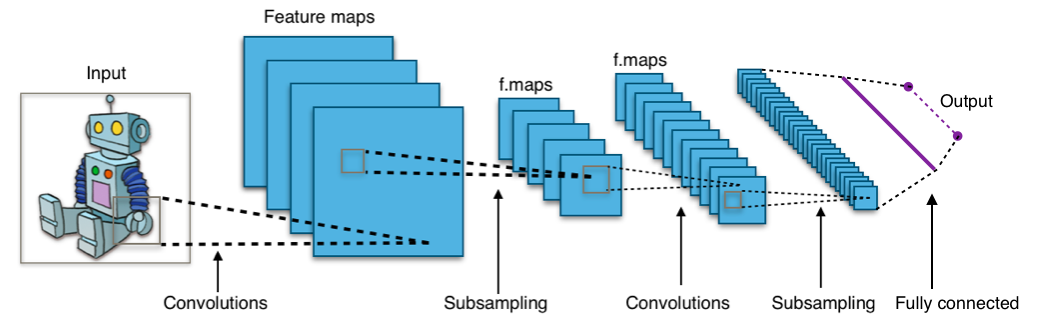
\includegraphics[width=\textwidth]{fig/CNN.png}    
    \caption{CNN architecture}
\end{figure}
\subsubsection{Siamese neural network}
A Siamese neural network is a type of neural network architecture that is commonly used for tasks related to similarity or distance-based learning.
It consist two or more identical subnetworks, each of them process two or more input data points and output a vector representation for each of them. 
The vector representations are then compared using a distance metric to determine the similarity between the input data points.

Siamese networks are widely used in tasks such as image or text matching.
They are particularly useful when dealing with small datasets or datasets with high variability, 
as they can learn to recognize patterns and similarities without requiring a large amount of data.
Figure 2. demonstrate the Siamese neural network.
\begin{figure}
    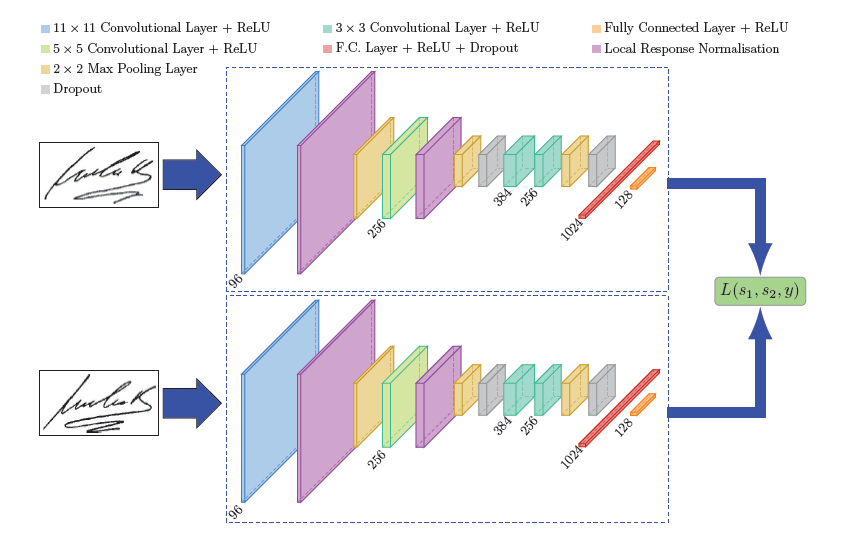
\includegraphics[width=\textwidth]{fig/SiameseNN.png}    
    \caption{CNN architecture}
\end{figure}
\section{Proposed Idea}
With the advancement of automated malware generationa and obfuscation, 
traditional detection to malware are gradually losing their effectiveness or applicability over time.
In \cite{ref1} \textit{Mingdong et al.} proposed an idea to extract API calls using dynamic analysis and then 
map it into feature image based on colour mapping rules. They trained a CNN model to classify 9 class of malware families.
and 1000 variants. Figure 3. shows the overview of dynamic API call malware detection.
\begin{figure}
    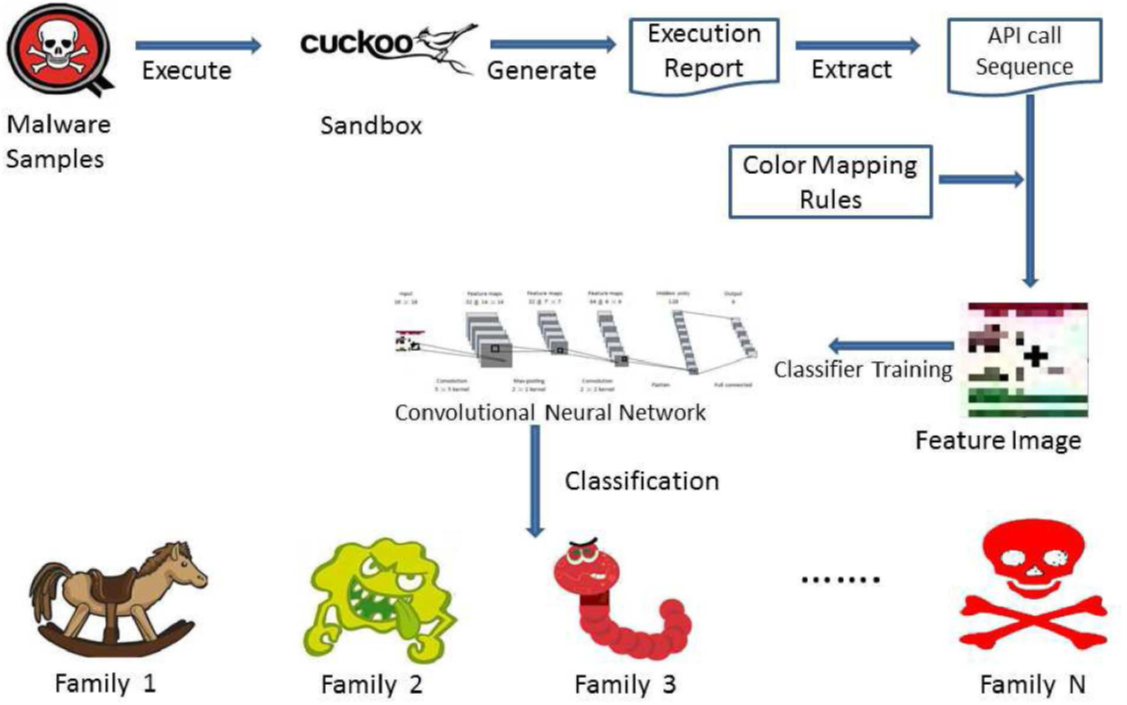
\includegraphics[width=\textwidth]{fig/overview.png}    
    \caption{CNN architecture}
\end{figure}
\subsection{Malware API extraction}
\subsection{Colour mapping rules}
\subsection{New idea}
To collect huge dataset for malware API call is not easy. To reduce the dataset demand for training neural network, 
we proposed and new idea that is to switch CNN into \textbf{Siamese neural network for few-shot training}.



\section{Expected Result}
Due to the challenges of collecting large and diverse datasets on rapid evolution of Malware, traditional Convolution Neural Network(CNNs) may struggle to fully show their strenths.As mention in our Related Work ,Siamese neural network have been widely using in image or text matching,and are known for their adaptability to small or High variability datasets.Therefore,based on our New idea we'll attempt to utilize Siamese neural networks with few shot learing to achieve a better accuracy then CNNs.
\begin{thebibliography}{99}  
    \bibitem{ref1}Mingdong Tang, Quan Qain.: 'Dynamic API call sequence visualisation for malware classification'. IET information security, 2019: 1751-8709.  
\end{thebibliography}
\end{document}